% Options for packages loaded elsewhere
\PassOptionsToPackage{unicode}{hyperref}
\PassOptionsToPackage{hyphens}{url}
%
\documentclass[
  man,floatsintext]{apa6}
\usepackage{amsmath,amssymb}
\usepackage{lmodern}
\usepackage{iftex}
\ifPDFTeX
  \usepackage[T1]{fontenc}
  \usepackage[utf8]{inputenc}
  \usepackage{textcomp} % provide euro and other symbols
\else % if luatex or xetex
  \usepackage{unicode-math}
  \defaultfontfeatures{Scale=MatchLowercase}
  \defaultfontfeatures[\rmfamily]{Ligatures=TeX,Scale=1}
\fi
% Use upquote if available, for straight quotes in verbatim environments
\IfFileExists{upquote.sty}{\usepackage{upquote}}{}
\IfFileExists{microtype.sty}{% use microtype if available
  \usepackage[]{microtype}
  \UseMicrotypeSet[protrusion]{basicmath} % disable protrusion for tt fonts
}{}
\makeatletter
\@ifundefined{KOMAClassName}{% if non-KOMA class
  \IfFileExists{parskip.sty}{%
    \usepackage{parskip}
  }{% else
    \setlength{\parindent}{0pt}
    \setlength{\parskip}{6pt plus 2pt minus 1pt}}
}{% if KOMA class
  \KOMAoptions{parskip=half}}
\makeatother
\usepackage{xcolor}
\usepackage{graphicx}
\makeatletter
\def\maxwidth{\ifdim\Gin@nat@width>\linewidth\linewidth\else\Gin@nat@width\fi}
\def\maxheight{\ifdim\Gin@nat@height>\textheight\textheight\else\Gin@nat@height\fi}
\makeatother
% Scale images if necessary, so that they will not overflow the page
% margins by default, and it is still possible to overwrite the defaults
% using explicit options in \includegraphics[width, height, ...]{}
\setkeys{Gin}{width=\maxwidth,height=\maxheight,keepaspectratio}
% Set default figure placement to htbp
\makeatletter
\def\fps@figure{htbp}
\makeatother
\setlength{\emergencystretch}{3em} % prevent overfull lines
\providecommand{\tightlist}{%
  \setlength{\itemsep}{0pt}\setlength{\parskip}{0pt}}
\setcounter{secnumdepth}{-\maxdimen} % remove section numbering
% Make \paragraph and \subparagraph free-standing
\ifx\paragraph\undefined\else
  \let\oldparagraph\paragraph
  \renewcommand{\paragraph}[1]{\oldparagraph{#1}\mbox{}}
\fi
\ifx\subparagraph\undefined\else
  \let\oldsubparagraph\subparagraph
  \renewcommand{\subparagraph}[1]{\oldsubparagraph{#1}\mbox{}}
\fi
\newlength{\cslhangindent}
\setlength{\cslhangindent}{1.5em}
\newlength{\csllabelwidth}
\setlength{\csllabelwidth}{3em}
\newlength{\cslentryspacingunit} % times entry-spacing
\setlength{\cslentryspacingunit}{\parskip}
\newenvironment{CSLReferences}[2] % #1 hanging-ident, #2 entry spacing
 {% don't indent paragraphs
  \setlength{\parindent}{0pt}
  % turn on hanging indent if param 1 is 1
  \ifodd #1
  \let\oldpar\par
  \def\par{\hangindent=\cslhangindent\oldpar}
  \fi
  % set entry spacing
  \setlength{\parskip}{#2\cslentryspacingunit}
 }%
 {}
\usepackage{calc}
\newcommand{\CSLBlock}[1]{#1\hfill\break}
\newcommand{\CSLLeftMargin}[1]{\parbox[t]{\csllabelwidth}{#1}}
\newcommand{\CSLRightInline}[1]{\parbox[t]{\linewidth - \csllabelwidth}{#1}\break}
\newcommand{\CSLIndent}[1]{\hspace{\cslhangindent}#1}
\ifLuaTeX
\usepackage[bidi=basic]{babel}
\else
\usepackage[bidi=default]{babel}
\fi
\babelprovide[main,import]{english}
% get rid of language-specific shorthands (see #6817):
\let\LanguageShortHands\languageshorthands
\def\languageshorthands#1{}
% Manuscript styling
\usepackage{upgreek}
\captionsetup{font=singlespacing,justification=justified}

% Table formatting
\usepackage{longtable}
\usepackage{lscape}
% \usepackage[counterclockwise]{rotating}   % Landscape page setup for large tables
\usepackage{multirow}		% Table styling
\usepackage{tabularx}		% Control Column width
\usepackage[flushleft]{threeparttable}	% Allows for three part tables with a specified notes section
\usepackage{threeparttablex}            % Lets threeparttable work with longtable

% Create new environments so endfloat can handle them
% \newenvironment{ltable}
%   {\begin{landscape}\centering\begin{threeparttable}}
%   {\end{threeparttable}\end{landscape}}
\newenvironment{lltable}{\begin{landscape}\centering\begin{ThreePartTable}}{\end{ThreePartTable}\end{landscape}}

% Enables adjusting longtable caption width to table width
% Solution found at http://golatex.de/longtable-mit-caption-so-breit-wie-die-tabelle-t15767.html
\makeatletter
\newcommand\LastLTentrywidth{1em}
\newlength\longtablewidth
\setlength{\longtablewidth}{1in}
\newcommand{\getlongtablewidth}{\begingroup \ifcsname LT@\roman{LT@tables}\endcsname \global\longtablewidth=0pt \renewcommand{\LT@entry}[2]{\global\advance\longtablewidth by ##2\relax\gdef\LastLTentrywidth{##2}}\@nameuse{LT@\roman{LT@tables}} \fi \endgroup}

% \setlength{\parindent}{0.5in}
% \setlength{\parskip}{0pt plus 0pt minus 0pt}

% Overwrite redefinition of paragraph and subparagraph by the default LaTeX template
% See https://github.com/crsh/papaja/issues/292
\makeatletter
\renewcommand{\paragraph}{\@startsection{paragraph}{4}{\parindent}%
  {0\baselineskip \@plus 0.2ex \@minus 0.2ex}%
  {-1em}%
  {\normalfont\normalsize\bfseries\itshape\typesectitle}}

\renewcommand{\subparagraph}[1]{\@startsection{subparagraph}{5}{1em}%
  {0\baselineskip \@plus 0.2ex \@minus 0.2ex}%
  {-\z@\relax}%
  {\normalfont\normalsize\itshape\hspace{\parindent}{#1}\textit{\addperi}}{\relax}}
\makeatother

% \usepackage{etoolbox}
\makeatletter
\patchcmd{\HyOrg@maketitle}
  {\section{\normalfont\normalsize\abstractname}}
  {\section*{\normalfont\normalsize\abstractname}}
  {}{\typeout{Failed to patch abstract.}}
\patchcmd{\HyOrg@maketitle}
  {\section{\protect\normalfont{\@title}}}
  {\section*{\protect\normalfont{\@title}}}
  {}{\typeout{Failed to patch title.}}
\makeatother

\usepackage{xpatch}
\makeatletter
\xapptocmd\appendix
  {\xapptocmd\section
    {\addcontentsline{toc}{section}{\appendixname\ifoneappendix\else~\theappendix\fi\\: #1}}
    {}{\InnerPatchFailed}%
  }
{}{\PatchFailed}
\keywords{language production, individual differences, cognitive skills, picture naming}
\usepackage{lineno}

\linenumbers
\usepackage{csquotes}
\raggedbottom
\usepackage{amsmath}
\usepackage{tipa}
\newfontfamily\PF{Arial}
\ifLuaTeX
  \usepackage{selnolig}  % disable illegal ligatures
\fi
\IfFileExists{bookmark.sty}{\usepackage{bookmark}}{\usepackage{hyperref}}
\IfFileExists{xurl.sty}{\usepackage{xurl}}{} % add URL line breaks if available
\urlstyle{same} % disable monospaced font for URLs
\hypersetup{
  pdftitle={Influences of cognitive skills and task difficulty on picture naming speed},
  pdfauthor={Pamela Fuhrmeister1, Sylvain Madec1, \& Audrey Bürki1},
  pdflang={en-EN},
  pdfkeywords={language production, individual differences, cognitive skills, picture naming},
  hidelinks,
  pdfcreator={LaTeX via pandoc}}

\title{Influences of cognitive skills and task difficulty on picture naming speed}
\author{Pamela Fuhrmeister\textsuperscript{1}, Sylvain Madec\textsuperscript{1}, \& Audrey Bürki\textsuperscript{1}}
\date{}


\shorttitle{Cognitive skills and picture naming}

\authornote{

This research was funded by the Deutsche Forschungsgemeinschaft (DFG, German Research Foundation) -- project number 317633480 -- SFB 1287, Project B05 (Bürki).

Correspondence concerning this article should be addressed to Pamela Fuhrmeister, Karl-Liebknecht-Straße 24-25 14476 Potsdam Germany. E-mail: \href{mailto:pamela.fuhrmeister@uni-potsdam.de}{\nolinkurl{pamela.fuhrmeister@uni-potsdam.de}}

}

\affiliation{\vspace{0.5cm}\textsuperscript{1} University of Potsdam, Department of Linguistics}

\abstract{%
Studies show a wide range of individual variability in the time it takes speakers to produce a word or short phrase (e.g., in picture naming tasks). This variability in language production has often been attributed to variability in cognitive skills, such as attention, working memory, or inhibition. However, these skills are not necessarily unitary constructs, and different tasks that measure a certain construct (e.g., inhibition) may measure different components of the skill. There is also some evidence (e.g., from dual-task paradigms) that the relationships between cognitive skills and language production are more apparent with more demanding production tasks. In two experiments, we examined the relationship between a variety of cognitive measures (thought to tap into different aspects of the cognitive skills they measure) and picture naming speed. In the second experiment, the role of task difficulty was also probed by manipulating the perceived amount of time participants were given to name a picture. In the first experiment, one significant correlation was found between a measure of cognitive skills (sustained attention) and picture naming speed; however, this was not replicated in the second experiment. We discuss the implications of these findings with respect to statisitcal power, reliability, and the specific tasks used to measure cognitive skills.
}



\begin{document}
\maketitle

Speaking is a well-practiced activity that, under many circumstances, feels fairly effortless. However, there is ample evidence that speaking does not necessarily happen automatically and may be at least partially dependent on available cognitive resources. For instance, speaking can interfere with a simultaneous task, such as driving a vehicle (e.g., Kubose et al., 2006) because it diverts cognitive resources away from driving (Strayer \& Johnston, 2001). Many laboratory studies of language production report a large amount of individual variability in how quickly speakers can, for example, name a picture (Bürki, 2017; Laganaro, Valente, \& Perret, 2012; Valente, Bürki, \& Laganaro, 2014), and this variability has been assumed to reflect differences in cognitive resources or abilities (e.g., Jongman, 2017; Jongman, Meyer, \& Roelofs, 2015; Jongman, Roelofs, \& Meyer, 2015; Piai \& Roelofs, 2013; Shao, Meyer, \& Roelofs, 2013; Shao, Roelofs, Acheson, \& Meyer, 2014; Shao, Roelofs, Martin, \& Meyer, 2015; Shao, Roelofs, \& Meyer, 2012; Sikora, Roelofs, Hermans, \& Knoors, 2016).

\hypertarget{cognitive-abilities-that-predict-speed-of-language-production}{%
\subsection{Cognitive abilities that predict speed of language production}\label{cognitive-abilities-that-predict-speed-of-language-production}}

Several studies have shown that how quickly an individual can produce words or short phrases is related to more general cognitive skills, including attention (Jongman, 2017; Jongman, Meyer, et al., 2015; Jongman, Roelofs, et al., 2015), working memory (Lorenz, Zwitserlood, Regel, \& Abdel Rahman, 2019; Piai \& Roelofs, 2013; Shao et al., 2012; but see Klaus \& Schriefers, 2018), and inhibition (Shao et al., 2013, 2014, 2015, 2012; Sikora et al., 2016). For the current study, we are interested in how generalizable these relationships are, specifically, whether we find similar relationships between picture naming speed and cognitive tasks when employing a wider battery of cognitive tests that are thought to measure these constructs. As we discuss in more detail in the next section, some tasks that have been used to measure certain cognitive skills do not necessarily correlate well with each other. For example, Flanker and Simon tasks are both thought to measure inhibition, but correlations between these measures are consistently low (e.g., Paap \& Sawi, 2014). A skill like inhibition (like other cognitive abilities) is not a unitary construct, and different tasks may very well tap into different types or components of inhibition.

This provides an opportunity to learn more about which aspects or components of inhibition, working memory, or attention are involved in language production. For instance, we ask whether scores on cognitive tasks performed in different domains (e.g., linguistic, non-linguistic, auditory, visual) thought to measure a similar construct or tasks that likely tap into different aspects of a skill similarly predict word production speed. In the following sections, we will give an overview of the cognitive functions (working memory, inhibition, and sustained attention) that have been found to correlate with language production speed, and we will discuss tasks that are often used to measure these constructs.

\hypertarget{working-memory}{%
\subsubsection{Working memory}\label{working-memory}}

Working memory can be described as the ability to hold information in mind and manipulate it in order to perform a cognitive task (e.g., Baddeley, 1992, 2010). Commonly used tasks to evaluate working memory include, for example, span tasks (e.g., Conway et al., 2005). In span tasks, participants are asked to remember target items whose presentation alternates with distractor items or another task. For instance, the operation span task consists of the alternating presentation of a letter and an arithmetic problem. Participants are asked to solve each math problem and to recall all letters at the end of a sequence (e.g., Unsworth, Heitz, Schrock, \& Engle, 2005). Given that this task requires the participant to recall verbal material, it is often used to determine whether participants' performance on a linguistic task correlates or is predicted by working memory scores. In other tasks, participants are asked to remember the positions of a shape on a grid (symmetry span task, e.g., Unsworth, Redick, Heitz, Broadway, \& Engle, 2009) or the length and directions of arrows (rotation span task, Harrison et al., 2013).

Shao et al. (2012) found a correlation between participants' performance on the operation span task and their speed of naming pictures of actions (though not pictures of objects), suggesting that working memory is at least partially involved with word production. However, as suggested by various authors (Conway et al., 2005; Engle, Tuholski, Laughlin, \& Conway, 1999; Shipstead, Redick, \& Engle, 2012), participants' scores on span tasks are not completely independent from the demands of the task. For instance, two participants with the same working memory capacities but different arithmetic skills will likely obtain different scores on the operation span task. Therefore, it is of interest to test whether other types of span tasks (e.g., rotation or symmetry) are also related to picture naming speed, as the demands of the distractor items in these tasks may influence participants' scores on the tasks. In the current study, we tested participants' working memory ability with three span task: the operation span, symmetry span, and rotation span tasks (see the Methods section for more details).

\hypertarget{inhibition}{%
\subsubsection{Inhibition}\label{inhibition}}

Inhibition is described as the ability to resolve conflicts and suppress irrelevant information. Recent studies, however, suggest that inhibition is not a unitary construct (Rey-Mermet \& Gade, 2018; Rouder \& Haaf, 2019). For instance, inhibition can be characterized as being selective or non-selective (Shao et al., 2013, 2015). Non-selective inhibition is the ability to inhibit any unwanted response (De Jong, Coles, \& Logan, 1995), while selective inhibition describes the ability to inhibit a more specific response that directly competes with the desired response (Forstmann et al., 2008). Several authors further subdivide selective inhibition into two different types: stimulus-stimulus conflict and stimulus-response conflict (Hommel, 1997; Kornblum, 1994; Scerrati, Lugli, Nicoletti, \& Umiltà, 2017). Stimulus-stimulus conflicts arise from an incompatibility between overlapping task-relevant and task-irrelevant features of the stimulus to be processed (e.g., in a Flanker task), while stimulus-response conflicts arise from an overlap of incongruent stimulus and response features (e.g., in a Simon task, Kornblum, 1994).

Measures of both selective and non-selective inhibition have been found to correlate with picture naming speed or the magnitude of experimental effects in a picture naming task (Shao et al., 2013, 2015). For instance, Shao et al. (2013) measured non-selective inhibition by means of a stop-signal reaction time task (Logan \& Cowan, 1984), which is thought to assess the ability to inhibit a motor response that has already been initiated, i.e., a non-linguistic response. On this task, participants are asked to respond to a stimulus presented, but on a certain proportion of the trials, they hear a tone to indicate they should withhold their response on that trial. Shao et al. (2012) and Shao et al. (2013) reported that participants' performance on the stop-signal reaction time task correlated with picture naming speed, suggesting that the relationship between language production and non-selective inhibition may not be specific to the language domain. However, this correlation was not replicated in Shao et al. (2015).

Shao et al. (2013, 2015) measured selective inhibition using a within-task measure derived from distributional properties of the task. In those studies, participants performed a picture-word interference task, in which they named pictures with printed distractor words overlayed on them. The distractor words were either semantically related or unrelated to the target word. Participants typically need more time to produce words when they see semantically related distractors than unrelated distractors (i.e., the semantic interference effect, see Bürki, Elbuy, Madec, \& Vasishth, 2020 for review). Shao et al. (2013, 2015) used the delta plot procedure (Ridderinkhof, Scheres, Oosterlaan, \& Sergeant, 2005; Ridderinkhof, Wildenberg, Wijnen, Burle, et al., 2004) to compute a measure of inhibition, which can be understood as the change in the semantic interference effect over the trials in the experiment with the slowest response times. Shao et al. (2013, 2015) found that this within-task measure of inhibition correlated with the magnitude of the semantic interference effect in a picture-word interference task, as well as in a semantic blocking task (Shao et al., 2015).

It is certainly intuitive that inhibition may be needed for a task such as the picture-word interference task and possibly language production more generally, as some theories of production assume lexical selection is a competitive process (e.g., Levelt, Roelofs, \& Meyer, 1999). However, we showed using simulated data that the correlation between this within-task measure of inhibition and the semantic interference effect arises as a mere consequence of the distributional properties of the data (Fuhrmeister \& Bürki, 2022). Specifically, the semantic interference effect is largest in the slowest responses; therefore, it is not surprising that this measure that is computed in part with the effect size over the slowest trials correlates strongly with the mean semantic interference effect. It is certainly possible that selective inhibition is involved in language production; however, we need different measures of inhibition to support this idea. Shao et al. (2014) have an additional study where participants named pictures with low and high name agreement (the number of possible names for pictures; low = more possible names). They found a more negative N2 (an electrophysiological component thought to reflect inhibition) for pictures with low name agreement, and with low name agreement, participants likely have to inhibit the other possible names for the picture.

In the present study, we used the stop-signal reaction time task to measure non-selective inhibition, as well as two different measures of selective inhibition (Flanker and Simon tasks) that, as discussed above, are thought to measure stimulus-stimulus (Flanker) and stimulus-response conflict (Simon) within the construct of selective inhibition (see the Methods section for more details).

\hypertarget{attention}{%
\subsubsection{Attention}\label{attention}}

Sustained attention describes the ability to maintain alertness to detect infrequent events over a long period of time (Sarter, Givens, \& Bruno, 2001). A common task to measure sustained attention is the continuous performance task, in which participants attend to a large number of stimuli and are asked to detect rare target stimuli. Several studies have found relationships between measures of sustained attention and language production (Jongman, Meyer, et al., 2015; Jongman, Roelofs, et al., 2015). For example, Jongman and colleagues have used variations of the continuous performance task with geometrical shapes (Jongman, Roelofs, et al., 2015) and digits (Jongman, Meyer, et al., 2015; Jongman, Roelofs, et al., 2015). In addition, Jongman, Roelofs, et al. (2015) have utilized both visual and auditory variations of this task and found that both variations correlated significantly with each other and with picture naming speed (Jongman, Roelofs, et al., 2015). This provides some evidence that relationships between sustained attention and language production measures may reflect more general attention abilities and may not be specific to a certain domain.

A disadvantage of the continuous performance task is that it generates very few errors (see e.g., Jongman, Roelofs, et al., 2015). For this reason, we chose a different sustained attention task for the present study, namely the continuous time expectancy task, which typically generates more errors (O'Connell et al., 2009). In this task, participants have to monitor a flow of alternating visual patterns and detect patterns that are presented for a longer duration than the others. In order to compare our results to previous findings (Jongman, Meyer, et al., 2015; Jongman, Roelofs, et al., 2015), we also asked participants to perform a conjunctive continuous performance task (Shalev, Ben-Simon, Mevorach, Cohen, \& Tsal, 2011). In this task, participants see a series of visual symbols in different shapes and colors, and their task is to respond when they see a specific shape with a specific color. Because participants have to pay attention to both shape and color, this task has been argued to increase attentional demands as compared to a continuous performance task (Shalev et al., 2011). We provide more details on these tasks in the Methods section.

\hypertarget{experiment-1}{%
\section{Experiment 1}\label{experiment-1}}

The goal of the current study is to extend previous findings on the relationship between cognitive skills and word production and to test how generalizable these relationships are. In the first experiment, participants performed a picture-word interference task, in which they named pictures with printed distractor words superimposed on the pictures. The task included several conditions: a baseline condition, in which participants saw a line of Xs printed on the picture; a semantic condition, in which participants saw a distractor that was either semantically related or unrelated to the picture; and a phonological condition, in which participants saw a distractor that was either phonologically related or unrelated to the target. The picture naming data have been reported elsewhere (Bürki \& Madec, 2022; Fuhrmeister, Madec, Lorenz, Elbuy, \& Bürki, 2022). For the present purposes, we analyzed only trials in the baseline condition to test whether measures of working memory, inhibition, or attention predict speed of simple picture naming.

\hypertarget{methods}{%
\section{Methods}\label{methods}}

\hypertarget{participants}{%
\subsection{Participants}\label{participants}}

A total of 45 participants (ages 18-30, mean age = 23, \emph{SD} = 3.51) were recruited for the study. All participants were native speakers of German and reported normal hearing and no history of psychiatric, neurological, or language disorders. Participants were paid or received course credit for their participation in the study, and they gave informed consent according to the University of Potsdam's (Germany) ethical committee guidelines.

\hypertarget{procedure}{%
\subsection{Procedure}\label{procedure}}

In the first session, participants completed a picture-word interference task, a delayed naming task, and a word reading task (i.e., reading aloud). Again, only the baseline condition of the picture-word interference task is reported here. The continuous EEG was also recorded during the picture-word interference task, but those data are also reported elsewhere (Fuhrmeister et al., 2022). In a subsequent session, participants performed the following cognitive tasks in this order to test for relationships between measures of cognitive functions and performance on the language production task (see also Table \ref{tab:cogskillsdesstats}): operation span, symmetry span, rotation span, continuous time expectancy task, Simon task, Flanker task, conjunctive continuous performance task, stop-signal reaction time task.\footnote{The following cognitive tests were also administered: the German MWT-B (Mehrfachwahl-Wortschatztest, Version B, Lehrl, 1975), the coding subtest of the Wechsler Adult Intelligence Scale--Fourth Edition (WAIS-IV, Wechsler, 2008), the digit span forward and backward subtest of the Wechsler Memory Scale Revised (Wechsler, 1987), and the Corsi block-tapping task forward and backward (Corsi, 1972). This battery of tests was used for an institutional project on variability in language to compare across age groups and to screen potential control participants for projects that involve participants with aphasia. These tests were not analyzed in the present study and will not be reported further.}

\hypertarget{stimuli-and-task-descriptions}{%
\subsection{Stimuli and task descriptions}\label{stimuli-and-task-descriptions}}

\hypertarget{picture-naming-task}{%
\subsubsection{Picture naming task}\label{picture-naming-task}}

Stimuli for the picture naming task consisted of 90 pictures from the Multipic database (Duñabeitia et al., 2018). Lemma frequencies (mean frequency = 1991.3, \emph{SD} = 3678.4, range 9-21184) for the words were obtained from the dlex database (Heister et al., 2011). As mentioned above, the original task contained several conditions with distractor words printed on the pictures; however, only trials from the baseline condition, which consisted of six Xs superimposed on the picture, are reported here.

Participants were first familiarized with the pictures: They saw one picture at a time on the screen with its corresponding name and were asked to read the words silently. The presentation of items was randomized.

For the picture naming task, participants first completed a short training phase, followed by the main task, which consisted of five blocks of trials. Each picture was presented once per block, and there was an equal number of trials in each condition per block. Pictures were presented in a pseudorandom order in each block. The structure of a trial was as follows: a fixation cross appeared on the screen for 2200-2300ms; then the picture was displayed either for 2300ms or until the participant started speaking. Vocal responses were recorded for 3000ms starting at the onset of picture presentation. A trial ended with an inter-trial interval that had a random duration between 1000 and 1200ms.

\hypertarget{cognitive-skills}{%
\subsubsection{Cognitive skills}\label{cognitive-skills}}

Following previous work on the relationship between language production and domain-general cognitive abilities, we included tasks to measure participants' working memory, sustained attention, and inhibition abilities. In order to replicate and extend previous findings in the language production literature, we included several tasks that have been used (or were similar to those that have been used) in previous studies. In addition, we included tasks that targeted different aspects of these cognitive skills.

\hypertarget{span-tasks}{%
\paragraph{Span tasks}\label{span-tasks}}

To measure participants' working memory abilities, we administrated three span tasks: operation span, symmetry span, and rotation span. Following the recommendations of Foster et al. (2015), we had participants complete two blocks of each span task\footnote{These tasks are available from the Georgia Tech Attention and Working Memory Lab website (\url{http://englelab.gatech.edu}). We used their scripts to implement the tasks in OpenSesame (Mathôt, Schreij, \& Theeuwes, 2012) for stimulus presentation.}. Recall that each task consists of sequences of target and distractor items, and participants are asked to respond to distractor items (e.g., solve a math problem). At the end of each sequence, participants attempted to recall all target items in the order they were presented.

As discussed in the introduction, the operation span task consists of target items (letters to be recalled) and distractor items (math problems). The target and distractor items are presented in alternating order, and participants are asked to recall the letters in the order they were presented. In the symmetry span task, a sequence consists of the alternating presentation of a 4x4 grid containing a single square and a geometrical shape that may or may not be symmetrical relative to the vertical axis. The positions of the squares in the 4x4 grid are the target items, and the symmetrical or asymmetrical geometrical shapes are the distractor items. After each geometrical shape, participants must determine whether the shape was symmetrical or not. At the end of each sequence, participants are asked to recall the positions of the squares in the 4x4 grid. In the rotation span task, a sequence consists of an arrow (long or short) pointing in one of eight possible directions and a rotated letter that can be vertically reversed or not. Arrow lengths and directions are the target items, and rotated letters are the distractor items. For each distractor item, participants must determine whether the letter was reversed or not. At the end of the sequence, participants are asked to recall the lengths and directions of the arrows.

To determine the length of a sequence in the span tasks, we followed recommendations from Draheim, Harrison, Embretson, and Engle (2018). In the operation span task, the length of a sequence varied from three to eight items; in the symmetry span task, from two to six items; and in the rotation span task, from two to five items. Each block contained sequences of all possible lengths, and each block was repeated for each task (i.e., two blocks total per task).

To compute span scores, we used the partial-credit unit scoring procedure as described in Conway et al. (2005). For this procedure, participants receive ``partial credit'' for any recalled target items in a sequence, which is computed as the proportion of correctly recalled target items in a sequence. For example, in a sequence with four items to recall, if the participant correctly recalls two, they would get a score of .5 for that sequence. The proportions of correctly recalled target items are then averaged together for each block. We administered two blocks of each task, so we computed the mean scores of the two blocks for each participant and each span task separately to enter into further analyses.

\hypertarget{stop-signal-reaction-time-task}{%
\paragraph{Stop-signal reaction time task}\label{stop-signal-reaction-time-task}}

As described briefly above, the stop-signal reaction time task is thought to measure non-selective inhibition, i.e., the suppression of any unwanted or irrelevant response (De Jong et al., 1995). In this task, participants are asked to respond to various stimuli (``go'' trials), but on some trials, they are asked to inhibit their response (``no-go'' trials).

During the go trials, a fixation cross was displayed for 250 ms at the center of the screen and then replaced by either the symbol ``\textless{}'' or the symbol ``\textgreater{}''. Participants were instructed to press a left keyboard key after the onset of the ``\textless{}'' symbol and a right keyboard key after the onset of the ``\textgreater{}'' symbol. During the no-go trials, a tone (750Hz, lasting 75 ms) sounded shortly after the onset of the visual symbols, indicating to the participants that they should not respond on these trials. This was an adaptive task: At the beginning of the procedure, the delay between the onset of the visual symbol and the onset of the tone (i.e., the stop signal delay) was 250 ms (i.e., the tone was played 250 ms after the onset of the visual symbol). The stop signal delay was then adjusted depending on the participant's performance. Following successful inhibition, the stop signal delay was increased by 50 ms. When participants failed to inhibit the response on a no-go trial, the stop signal delay was reduced by 50 ms.

Following the recommendations of Matzke, Verbruggen, and Logan (2018), the task started with a familiarization block of 20 go trials. Then, participants performed a practice block with 18 go trials and 6 no-go trials. For this practice block, participants were instructed to not slow down their responses on go trials (Matzke et al., 2018). Three experimental blocks followed, consisting of 48 go trials and 16 no go trials. Participants were asked to perform the task as quickly as possible.

We computed scores on the stop signal reaction time task using the integration method (Verbruggen, Chambers, \& Logan, 2013). To do this, we first ordered the participants' reaction times on go trials from fastest to slowest. We then identified the reaction time that corresponded to the nth percentile, where n is defined as the percentage of the no-go trials that the participant incorrectly responded to (see also Hedge, Powell, \& Sumner, 2018 for a clear description of this procedure). For example, if a participant incorrectly responded on 40\% of the no-go trials, we would compute the 40th percentile of their reaction time distribution of go trials. Finally, we subtracted the mean stop signal delay from the nth reaction time. We carried out this procedure per participant and experimental block and then computed the mean score over the three experimental blocks for each participant and entered this score into further analyses. Reaction times are reported in milliseconds.

\hypertarget{flanker-task}{%
\paragraph{Flanker task}\label{flanker-task}}

To measure selective inhibition due to stimulus-stimulus conflict, participants completed a Flanker task. In this task, an arrow pointing either to the left or to the right is presented at the center of the screen, and participants have to determine the direction of the arrow using the corresponding left or right arrow key on the keyboard. This central arrow is flanked either by arrows pointing in the same direction (\(>>>>>\), congruent condition), the opposite direction (\(<<><<\), incongruent condition), or by straight lines (\(-->--\), neutral condition). Participants started with 18 training trials, six in each condition. There were four experimental blocks, each consisting of 46 congruent trials, 46 incongruent trials and 46 neutral trials (see Hedge et al., 2018 for justification regarding the number of trials in this task).

For each participant, we computed a measure of reaction time cost in milliseconds. We first removed trials with incorrect responses. Then we computed the reaction time cost by subtracting each participant's mean reaction time of the congruent trials from their mean reaction time of the incongruent trials.

\hypertarget{simon-task}{%
\paragraph{Simon task}\label{simon-task}}

The Simon is also a task thought to measure selective inhibition but the inhibition in this task is due to stimulus-response conflict. In the task we administered, participants saw either a blue or red circle on either the left- or right-hand side of a computer screen. Their task was to press a key on the left-hand side of the keyboard upon seeing a blue circle and on the right-hand side upon seeing a red circle, and they were asked to respond as quickly as possible. Trials with the blue circle appearing on the left-hand side or with a red circle appearing on the right-hand side are called congruent trials, because the position of the circle and the correct response key are on the same side. Conversely, trials where the blue circle appears on the right-hand side of the screen or a red circle on the left-hand side are called incongruent trials.

Participants started with a familiarization phase of 40 trials. During this phase, a blue (50\% of trials) or red circle appeared in the center of the screen, and they were asked to press the corresponding key on the keyboard. Then participants completed a practice phase with 56 trials. A trial started with the presentation of a fixation cross located at the center of the screen for 500ms. Then a blue or red circle appeared either on the left-hand or right-hand side of the fixation cross, and participants were instructed to indicate their response with the appropriate key. During this practice phase, there were 42 congruent trials (21 blue and 21 red circles), and 12 incongruent trials (6 blue and 6 red circles). After the practice phase, participants performed the same task in two experimental blocks of 120 trials each, with 90 congruent trials and 30 incongruent trials (see Wöstmann et al., 2013 on the selection of the number of trials).

The procedure for computing the reaction time cost was the same as for the Flanker task.

\hypertarget{conjunctive-continuous-performance-task}{%
\paragraph{Conjunctive continuous performance task}\label{conjunctive-continuous-performance-task}}

In this sustained attention task, participants see a flow of visual symbols that vary in shapes (i.e.~squares, triangles, stars, circles) and in color (i.e.~blue, green, red, yellow). Participants must press a button as soon as they see a red square. We followed the procedure outlined in Shalev et al. (2011). The task included 320 trials: 30\% of trials contained the target (i.e., the red square); 17.5\% of trials contained red, non-square symbols; 17.5\% of trials contained square, non-red symbols, and the remainder of the trials contained non-red and non-square symbols. The inter-trial interval ranged from 1000 ms to 2500 ms, by steps of 500 ms.

We calculated the hit rate for each participant, which was the proportion of target trials that the participant correctly responded to.

\hypertarget{continuous-time-expectancy-task}{%
\paragraph{Continuous time expectancy task}\label{continuous-time-expectancy-task}}

For this second task measuring sustained attention, participants saw visual patterns and were asked to identify a pattern that was presented for a longer duration than the others. We used four visual patterns, as in O'Connell et al. (2009). The standard duration in our task was set to 800ms, and the target duration was set to 1300ms. The procedure started with a familiarization block, followed by a training block, and ended with a single experimental block. During the familiarization block, 32 patterns appeared one by one on the screen. Four of these patterns were target patterns, while the other ones were standard patterns. Participants had to detect the target patterns but were not asked to respond. A training block followed only if participants reported that, during the familiarization block, they noticed some patterns (the target) lasting longer than the other ones. During the training block, they were instructed to press the space bar as soon as they noticed a target. There were 24 trials and among them, 3 targets. If participants were unable to detect the three targets during the training block, they had to perform it again until they were able to detect every target. The experimental block consisted in 674 trials, with 84 targets. Distances between two deviant trials ranged from 4 to 10 trials, with 12 trials for each of these numbers. Following the presentation of a target, participants had to provide an answer within 700ms.

We again calculated the hit rate for each participant, which was the proportion of target trials that the participant correctly responded to.

\hypertarget{analyses}{%
\subsection{Analyses}\label{analyses}}

\hypertarget{picture-naming-measures-and-correlations}{%
\subsubsection{Picture naming measures and correlations}\label{picture-naming-measures-and-correlations}}

To derive measures of picture naming speed, we estimated ex-gaussian parameters of each participant's response time distribution, following previous work (Jongman, Meyer, et al., 2015; Jongman, Roelofs, et al., 2015; Shao et al., 2013). An ex-gaussian distribution often provides a good fit to reaction time data and is composed of three parameters: mu (\(\mu\)), sigma (\(\sigma\)), and tau (\(\tau\)). The \(\mu\) and \(\sigma\) parameters represent the mean and standard deviation of the Gaussian portion of the distribution, respectively, and the \(\tau\) parameter represents the mean and standard deviation of the exponential part of the distribution (Balota \& Yap, 2011; Tse, Balota, Yap, Duchek, \& McCabe, 2010). The \(\tau\) parameter can be understood conceptually as the proportion of abnormally slow responses, or the right tail of the reaction time distribution. We estimated ex-gaussian parameters for each participant separately using the mexgauss() function in the retimes package (Massidda \& Massidda, 2013) in R (R Core Team, 2021). Only correct responses were included in the analyses of picture naming data.

We then tested for correlations between the ex-gaussian parameters \(\mu\) and \(\tau\) and measures of cognitive skills (\(\mu\) and \(\tau\) because we do not have theoretical motivation to think that we should find relationships between cognitive skills and variance). We acknowledge that this approach leads to a number of statistical tests being done, which can inflate Type I error rates. However, because we do not know which cognitive tests these relationships will generalize to, it is important to fully explore these relationships. Therefore we view Experiment 1 as an exploratory endeavor, in which we will first pinpoint plausible extensions of the relationships found previously in the literature by reporting correlations without correcting for multiple comparisons. We will replicate relationships found in Experiment 1 in a confirmatory manner in Experiment 2. All analyses were performed in R (R Core Team, 2021), and pre-processed data and analysis scripts are publicly available in the OSF repository at \url{https://osf.io/4ftex/}.

\begin{table}

\caption{\label{tab:cogskillsdesstats}Mean and standard deviation (sd) of scores on all cognitive tests.}
\centering
\begin{tabular}[t]{llrr}
\toprule
\em{Test} & \em{Skill being measured} & \em{mean} & \em{sd}\\
\midrule
Conjunctive continuous
 performance & Sustained attention & 1.00 & 0.01\\
Continuous time
 expectancy & Sustained attention & 0.82 & 0.15\\
Flanker RT cost & Selective inhibition & 63.47 & 21.73\\
Operation Span & Working memory & 0.75 & 0.16\\
Rotation Span & Working memory & 0.77 & 0.15\\
\addlinespace
Simon RT cost & Selective inhibition & 63.95 & 26.62\\
Stop-signal reaction time & Non-selective inhibition & 207.41 & 47.63\\
Symmetry Span & Working memory & 0.73 & 0.13\\
\bottomrule
\end{tabular}
\end{table}

\hypertarget{results}{%
\section{Results}\label{results}}

\hypertarget{descriptive-statistics}{%
\subsection{Descriptive statistics}\label{descriptive-statistics}}

We first calculated descriptive statistics (mean and standard deviation) of all of the cognitive measures to determine whether there is a sufficient amount of variability among participants to obtain meaningful correlations with each of the measures. In Table \ref{tab:cogskillsdesstats} we report the mean and standard deviation of each of the measures, and a histogram of the scores can be seen in Figure \ref{fig:exp1hist}. Visual inspection of the histograms suggests a ceiling effect for the conjunctive continuous performance task, which is confirmed by the descriptive statistics (\emph{M} = 1.00, \emph{SD} = 0.01). Due to this ceiling effect, we would not expect to be able to find meaningful correlations with this measure, so we do not consider it in any further analyses. All other measures seem to have a sufficient spread of scores to use in further analyses.



\begin{figure}
\centering
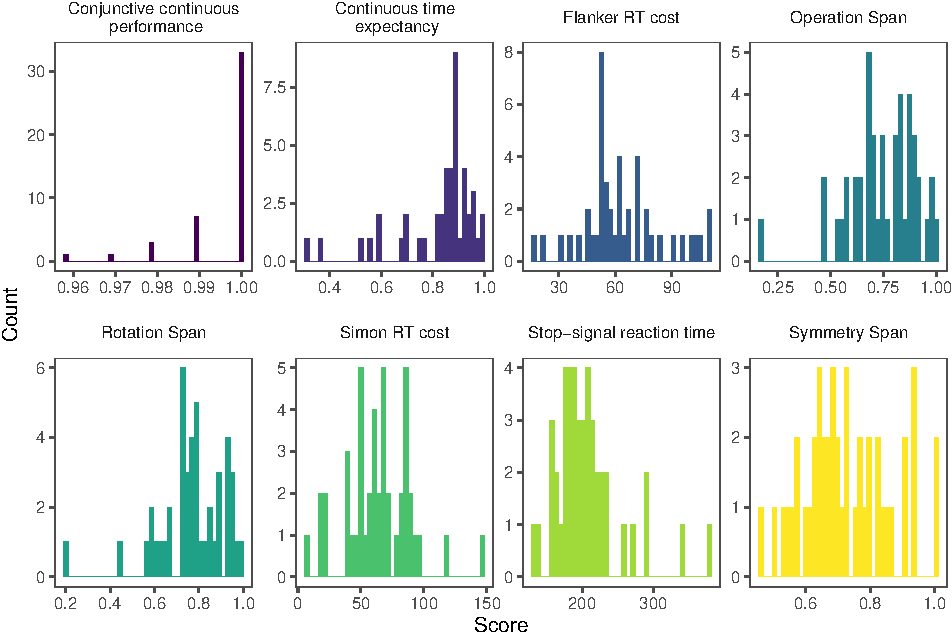
\includegraphics{task_difficulty_ind_dif_files/figure-latex/exp1hist-1.pdf}
\caption{\label{fig:exp1hist}Histogram of participants' scores on all cognitive tests. Note the difference in axes.}
\end{figure}

\hypertarget{correlations-among-measures-of-cognitive-skills}{%
\subsection{Correlations among measures of cognitive skills}\label{correlations-among-measures-of-cognitive-skills}}

Next, we report correlations among all measures to determine whether the cognitive tests thought to measure similar constructs are correlated with each other. Based on previous literature, we expected to find correlations among the inhibition measures (Simon, Flanker, and stop-signal reaction time tasks) and working memory measures (operation, symmetry, and rotation span tasks). However, some previous work has not found correlations among tasks thought to measure similar skills, such as inhibition (e.g., Paap \& Sawi, 2014); therefore, we may see only weak or no correlations among these skills. Figure \ref{fig:cogskillscor} reports correlations between all pairs of tasks. The span tasks correlated fairly well with each other, and there was also a significant correlation between the stop-signal reaction time task and the symmetry span task.



\begin{figure}
\centering
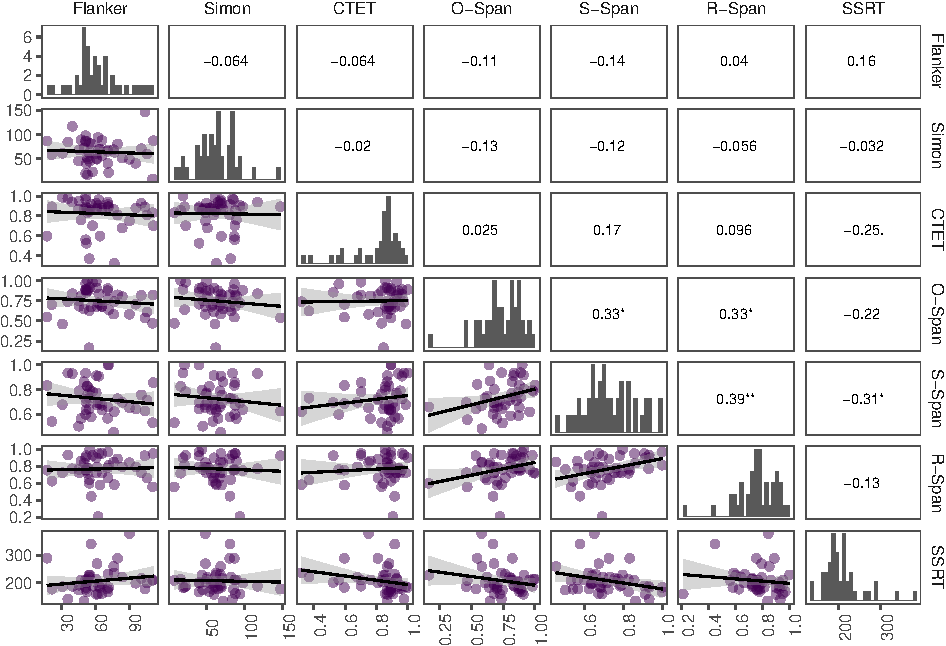
\includegraphics{task_difficulty_ind_dif_files/figure-latex/cogskillscor-1.pdf}
\caption{\label{fig:cogskillscor}Correlations between all cognitive measures in Experiment 1. Flanker = Flanker RT cost, Simon = Simon RT cost, CTET = continuous time expectancy task, O-Span = operation span task, S-Span = symmetry span task, R-Span = rotation span task, SSRT = stop-signal reaction time task. Significance levels: *** = \textless{} .001, ** = .01, * = .05, . = .1}
\end{figure}

\hypertarget{correlations-between-cognitive-skills-and-picture-naming-speed}{%
\subsection{Correlations between cognitive skills and picture naming speed}\label{correlations-between-cognitive-skills-and-picture-naming-speed}}

\begin{table}

\caption{\label{tab:cormutau}Correlations (r and p values) between cognitive skills and mu and tau parameters of picture naming response time distributions. Flanker = Flanker RT cost, Simon = Simon RT cost, CTET = continuous time expectancy task, O-Span = operation span task, S-Span = symmetry span task, R-Span = rotation span task, SSRT = stop-signal reaction time task.}
\centering
\begin{tabular}[t]{lrrrr}
\toprule
\em{ } & \em{mu r} & \em{mu p} & \em{tau r} & \em{tau p}\\
\midrule
Flanker & -0.06 & 0.69 & 0.14 & 0.36\\
Simon & 0.11 & 0.49 & 0.04 & 0.78\\
CTET & -0.20 & 0.18 & -0.29 & 0.06\\
O-Span & -0.07 & 0.66 & 0.01 & 0.96\\
S-Span & -0.06 & 0.70 & 0.11 & 0.47\\
\addlinespace
R-Span & -0.15 & 0.32 & 0.00 & 0.99\\
SSRT & 0.09 & 0.55 & 0.19 & 0.22\\
\bottomrule
\end{tabular}
\end{table}

The correlations between the ex-gaussian parameters and measures of cognitive skills can be found in Table \ref{tab:cormutau}. Only the continuous time expectancy task correlated significantly with the \(\mu\) parameter (i.e., the mean) suggesting that higher scores on the sustained attention task corresponded to faster naming speed. No correlations were found between cognitive skills and \(\tau\) (exponential).

\hypertarget{discussion}{%
\section{Discussion}\label{discussion}}

In Experiment 1, we tested whether several cognitive skills thought to be related to individual differences in language production correlated with other related measures (that perhaps tap into different aspects of these skills). We additionally tested whether any of these measures correlated with the \(\mu\) and \(\tau\) (exgaussian) parameters of the distribution of response times in a picture naming task.

We first found significant correlations among the span tasks that measure working memory. However, the inhibition measures did not seem to pattern all that similarly, with some correlations close to zero. We did not have enough variability in the conjunctive continuous performance task that measures attention to test for a correlation with the other measure of attention (continuous time expectancy task).

We also observed a significant correlation between the \(\mu\) parameter of the picture naming response time distribution and the continuous time expectancy task. This echos findings from previous work suggesting that better scores on sustained attention tasks predict faster response times in picture naming tasks (Jongman, 2017; e.g., Jongman, Meyer, et al., 2015; Jongman, Roelofs, et al., 2015); however, those relationships were mainly found with the \(\tau\) parameter, especially in comparable (simple) picture naming tasks (Jongman, 2017; Jongman, Roelofs, et al., 2015). In previous work, correlations between attention measures and the \(\tau\) parameter have been taken as evidence that participants with poorer sustained attention abilities have more trials with longer responses, perhaps due to more frequent lapses of attention during the task. The correlation we found with \(\mu\) however, suggests that participants with better sustained attention abilities were overall faster at picture naming. We note that the correlation barely reached significance (\emph{p} = .04), so we will hold off on interpreting this relationship further until it has been replicated.

\hypertarget{experiment-2}{%
\section{Experiment 2}\label{experiment-2}}

In Experiment 2, we test whether certain cognitive skills predict picture naming speed when participants are encouraged to respond faster, and we compare this with a non-speeded condition.

In Experiment 1, we found little support for the idea that cognitive skills predict picture naming latencies. However, the picture naming task was quite simple, and cognitive skills or resources may be more important when the task is more difficult. Some evidence for this idea comes from studies using a dual-task paradigm (e.g., Ferreira \& Pashler, 2002; Jongman, Roelofs, et al., 2015). For example, Piai and Roelofs (2013) had participants perform picture naming and tone discrimination tasks in a dual-task paradigm. They found a relationship between a measure of updating ability (i.e., working memory, as measured by an operation span task) and participants' picture naming speed, as well as the interference effect from the dual task: Participants with better updating or working memory abilities were faster to name pictures and were not as affected by the interference from the two tasks. Shao et al. (2012) similarly found evidence that cognitive skills are related to picture naming speed in more demanding task conditions. For example, updating ability (also measured by an operation span task) was correlated with picture naming speed for pictures of actions but not objects. They argue that naming pictures of actions is more difficult than naming pictures of objects because actions are conceptually and grammatically more complex.

The goal of Experiment 2 is to test whether relationships between cognitive skills and word production speed are stronger when the task is more difficult. In the current study, we manipulated task difficulty by decreasing the perceived amount of time that participants have to name a picture.

If more difficult tasks place higher cognitive demands on participants, we predict that better performance on cognitive skills will predict faster response times during the picture naming task in the speeded condition. We may see similar relationships in the non-speeded condition, but we expect that these relationships will be stronger in the speeded than in the non-speeded condition. Additionally, the non-speeded condition in Experiment 2 will serve as a replication of Experiment 1.

\hypertarget{methods-1}{%
\section{Methods}\label{methods-1}}

\hypertarget{participants-1}{%
\subsection{Participants}\label{participants-1}}

A total of 48 participants (ages 18-20, \emph{M} = 23.2, \emph{SD} = 3.5) took part in the experiment. All participants were right-handed, native speakers of German with typical hearing and no history of neurological or language disorders. Participants were either paid for their participation or received course credit. Participants were given details about the experimental procedure and gave informed consent before starting the experiment. The study received ethical approval by the ethical committee of the University of Potsdam (Germany).

\hypertarget{procedure-1}{%
\subsection{Procedure}\label{procedure-1}}

The experiment was conducted in two sessions. In the first session, participants completed a picture-word interference task and three related tasks: a recall task, a delayed naming task, and a word reading task; only the baseline trials from the picture-word interference task are reported here. In the second session, participants completed the same battery of cognitive tests administered in Experiment 1.

\hypertarget{stimuli-and-task-descriptions-1}{%
\subsection{Stimuli and task descriptions}\label{stimuli-and-task-descriptions-1}}

\hypertarget{picture-naming-task-1}{%
\subsubsection{Picture naming task}\label{picture-naming-task-1}}

To test whether cognitive skills are more strongly related to word production speed in more difficult tasks, participants performed picture-word interference task (as described in Experiment 1) under two conditions: a speeded and a non-speeded condition. Again, only the baseline trials (with Xs) were included in the analyses of the present experiment. The experiment consisted of two blocks, and each condition was administered in one block. Participants named two lists of pictures: Each list consisted of 20 training trials, 110 filler trials, and 225 test trials (order of condition and presentation of lists were counterbalanced). The structure of each block was as follows: Participants were first familiarized with the pictures and corresponding words that were used in that block of the task. Participants saw each picture displayed with its name in written form, and they were asked to read the name silently and to press a button to advance to the next picture. Participants were told they would be asked to name the pictures using the name from the familiarization phase in a later phase of the experiment. Next, participants completed a short training phase that consisted of 20 trials; training trials were not included in the analyses.

After the training phase, participants completed the main picture-word interference task. On each trial, a fixation cross was displayed on the screen for 800ms, and then the picture appeared. Participants were instructed to produce the name of the picture as fast as possible. The duration for which the item stayed on the screen depended on the experimental condition. Each block contained filler and test trials, and condition (speeded vs.~non-speeded) was manipulated with the filler trials only. In each block (both speeded and non-speeded), the picture on each test trial stayed on the screen for 1200ms, but the duration varied for the filler trials. In the non-speeded condition, the pictures on the filler trials stayed on the screen for 1200ms, just like the test trials. However, in the speeded condition, the pictures on the filler trials stayed on the screen for a shorter duration that varied between 400 and 600ms. Only the test trials were analyzed; the purpose of the filler trials was to manipulate the perceived amount of time that participants were given to name the picture. This ensured that the naming latencies that were compared across blocks were based on the same type of trials.

\hypertarget{cognitive-skills-1}{%
\subsubsection{Cognitive skills}\label{cognitive-skills-1}}

We used the same battery of cognitive tests that were used in Experiment 1 and computed scores in the same way.

\hypertarget{analyses-1}{%
\subsection{Analyses}\label{analyses-1}}

The analyses were identical to Experiment 1, except the exgaussian parameters were calculated for each condition (speeded vs.~non-speeded) separately. Again, only trials with correct responses in the picture naming task were included in the analyses. We report descriptive statistics, correlations of cognitive measures with each other, a comparison of response times in the speeded and non-speeded conditions, and finally, correlations between cognitive measures and \(\mu\) and \(\tau\) parameters from the response time distribution.

\hypertarget{results-1}{%
\section{Results}\label{results-1}}

\begin{table}

\caption{\label{tab:cogskillsdesstatsE2}Mean and standard deviation (sd) of scores on all cognitive tests.}
\centering
\begin{tabular}[t]{llrr}
\toprule
\em{Test} & \em{Skill being measured} & \em{mean} & \em{sd}\\
\midrule
Conjunctive continuous
 performance & Sustained attention & 98.13 & 5.08\\
Continuous time
 expectancy & Sustained attention & 0.80 & 0.20\\
Flanker RT cost & Selective inhibition & 75.39 & 32.86\\
Operation Span & Working memory & 0.79 & 0.15\\
Rotation Span & Working memory & 0.75 & 0.12\\
\addlinespace
Simon RT cost & Selective inhibition & 70.99 & 33.04\\
Stop-signal reaction time & Non-selective inhibition & 182.63 & 65.70\\
Symmetry Span & Working memory & 0.73 & 0.11\\
\bottomrule
\end{tabular}
\end{table}

\hypertarget{descriptive-statistics-1}{%
\subsection{Descriptive statistics}\label{descriptive-statistics-1}}

We first report descriptive statistics on all cognitive measures. Similar to Experiment 1, we want to ensure we have enough variability among participants to find meaningful correlations with the measures. Means and standard deviations for each measure can be found in Table \ref{tab:cogskillsdesstatsE2}, and histograms in Figure \ref{fig:exp2hist}. Similar to Experiment 1, we see a ceiling effect for the conjunctive continuous performance task (\emph{M} = 98.13, \emph{SD} = 5.08), although there is slightly more variability than in Experiment 1. This is mostly due to one participant who has a much lower score; however, this participant did not consistently score low on all measures; therefore, we assume the participant was indeed doing the tasks in good faith. As in Experiment 1, we will not include this measure in the following analyses.



\begin{figure}
\centering
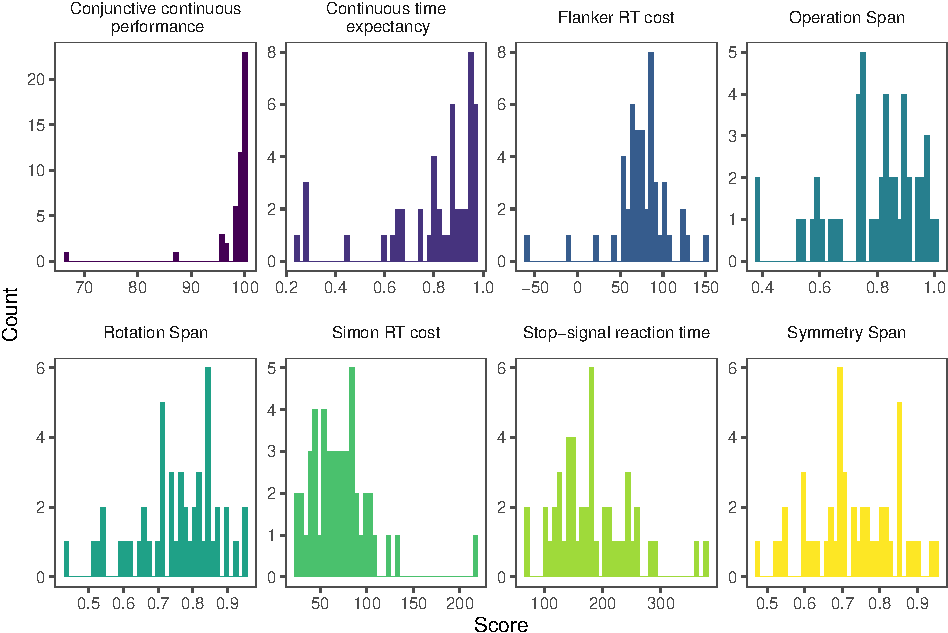
\includegraphics{task_difficulty_ind_dif_files/figure-latex/exp2hist-1.pdf}
\caption{\label{fig:exp2hist}Histogram of participants' scores on all cognitive tests. Note the difference in axes.}
\end{figure}

\hypertarget{correlations-among-measures-of-cognitive-skills-1}{%
\subsection{Correlations among measures of cognitive skills}\label{correlations-among-measures-of-cognitive-skills-1}}

Next, we computed the correlations of all the cognitive measures with each other, just as we did in Experiment 1. All correlations can be found in Figure \ref{fig:cogskillscorE2}. Here we see more significant correlations: The working memory (span task) measures patterned together again, the continuous time expectancy task correlated moderately with the span tasks, and the stop-signal reaction time task correlated with the Simon task (another measure of inhibition), as well as two of the span tasks.



\begin{figure}
\centering
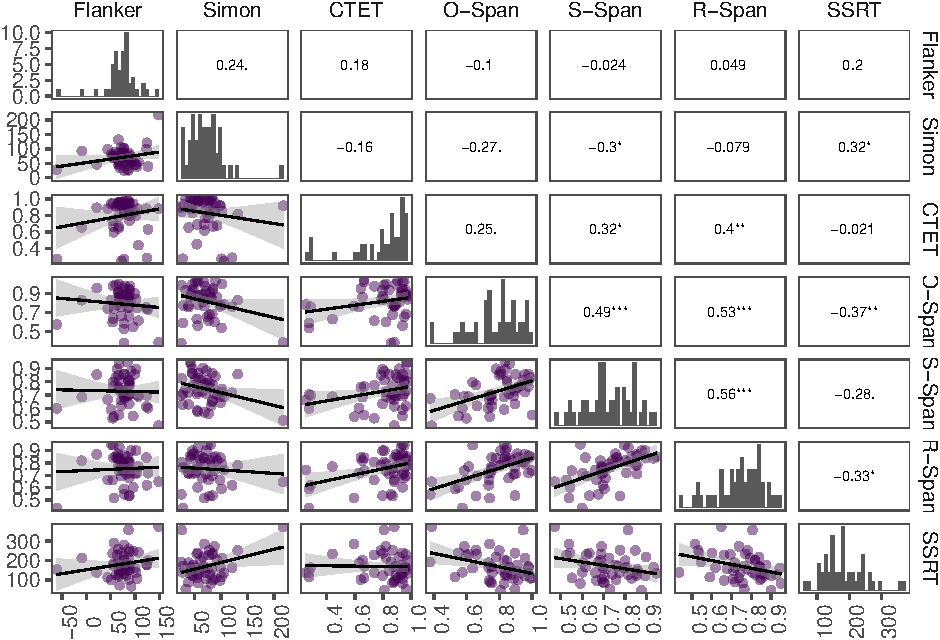
\includegraphics{task_difficulty_ind_dif_files/figure-latex/cogskillscorE2-1.pdf}
\caption{\label{fig:cogskillscorE2}Correlations between all cognitive measures in Experiment 2. Flanker = Flanker RT cost, Simon = Simon RT cost, CTET = continuous time expectancy task, O-Span = operation span task, S-Span = symmetry span task, R-Span = rotation span task, SSRT = stop-signal reaction time task. Significance levels: *** = \textless{} .001, ** = .01, * = .05, . = .1}
\end{figure}

\hypertarget{naming-latencies-in-the-speeded-and-non-speeded-conditions}{%
\subsection{Naming latencies in the speeded and non-speeded conditions}\label{naming-latencies-in-the-speeded-and-non-speeded-conditions}}

Because we only manipulated the perceived amount of time participants had to respond in the speeded condition, we first wanted to make sure that this manipulation did indeed encourage participants to respond faster. To test this, we fit a linear mixed effects model that predicted response time on the millisecond scale.\footnote{We also fit a model that predicted response time on the log scale and the results were similar.} The model included a fixed effect of speed condition (deviation coded: speeded = -.5, non-speeded = .5), by-participant random intercepts and slopes for speed condition, and by-item random intercepts. Results are displayed in Table \ref{tab:exp2speed} and Figure \ref{fig:exp2speedfig}. There was a significant main effect of speed condition, with responses being about 36ms faster in the speeded condition. This suggests that our manipulation did indeed encourage participants to respond faster in the speeded condition.

\begin{table}

\caption{\label{tab:exp2speed}Model comparing picture naming latencies in the speeded and non-speeded conditions on the millisecond scale. Responses in the non-speeded condition were about 36ms slower than in the speeded condition.}
\centering
\begin{tabular}[t]{lrrrl}
\toprule
\em{Predictor} & \em{Estimate} & \em{SE} & \em{t} & \em{p}\\
\midrule
Intercept & 678 & 10 & 68.03 & <.001\\
Speed Condition & 36 & 8 & 4.73 & <.001\\
\bottomrule
\end{tabular}
\end{table}



\begin{figure}
\centering
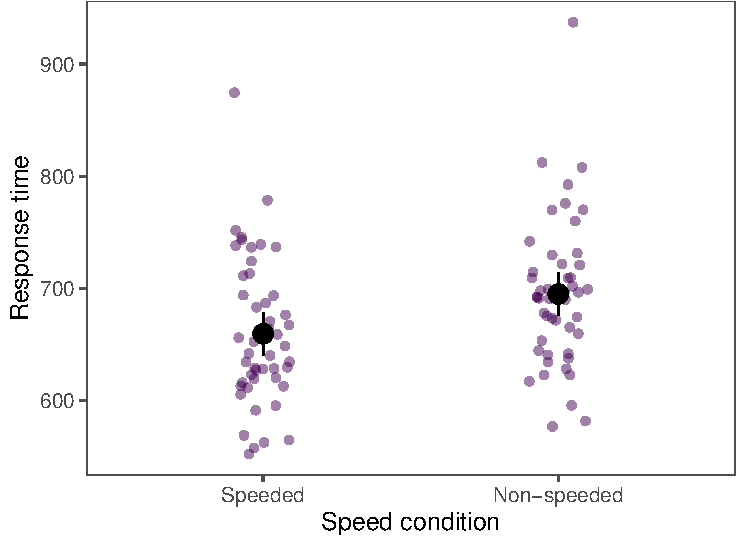
\includegraphics{task_difficulty_ind_dif_files/figure-latex/exp2speedfig-1.pdf}
\caption{\label{fig:exp2speedfig}Speed of responses on the picture naming task in the speeded and non-speeded conditions.}
\end{figure}

\begin{table}

\caption{\label{tab:cormutauE2}Correlations between cognitive skills (r and p values) and mu and tau parameters of picture naming response time distributions in the non-speeded condition of Experiment 2. Flanker = Flanker RT cost, Simon = Simon RT cost, CTET = continuous time expectancy task, O-Span = operation span task, S-Span = symmetry span task, R-Span = rotation span task, SSRT = stop-signal reaction time task.}
\centering
\begin{tabular}[t]{lrrrr}
\toprule
\em{ } & \em{mu r} & \em{mu p} & \em{tau r} & \em{tau p}\\
\midrule
Flanker & -0.22 & 0.14 & 0.00 & 1.00\\
Simon & 0.01 & 0.93 & 0.21 & 0.16\\
CTET & -0.15 & 0.32 & 0.05 & 0.75\\
O-Span & 0.13 & 0.36 & -0.24 & 0.10\\
S-Span & -0.04 & 0.77 & 0.12 & 0.43\\
\addlinespace
R-Span & 0.11 & 0.46 & -0.11 & 0.45\\
SSRT & 0.02 & 0.89 & 0.17 & 0.24\\
\bottomrule
\end{tabular}
\end{table}

\hypertarget{correlations-between-cognitive-skills-and-picture-naming-speed-1}{%
\subsection{Correlations between cognitive skills and picture naming speed}\label{correlations-between-cognitive-skills-and-picture-naming-speed-1}}

Finally, we tested the correlations between the mu and tau parameters of the picture naming response time distributions and the measures of cognitive skills. Results from the non-speeded task can be found in Table \ref{tab:cormutauE2}, and results from the speeded task are shown in Table \ref{tab:cormutauE2s}. We did not find any significant correlations in either condition.

\begin{table}

\caption{\label{tab:cormutauE2s}Correlations between cognitive skills (r and p values) and mu and tau parameters of picture naming response time distributions in the speeded condition of Experiment 2. Flanker = Flanker RT cost, Simon = Simon RT cost, CTET = continuous time expectancy task, O-Span = operation span task, S-Span = symmetry span task, R-Span = rotation span task, SSRT = stop-signal reaction time task.}
\centering
\begin{tabular}[t]{lrrrr}
\toprule
\em{ } & \em{mu r} & \em{mu p} & \em{tau r} & \em{tau p}\\
\midrule
Flanker & -0.03 & 0.82 & -0.16 & 0.28\\
Simon & 0.19 & 0.21 & 0.14 & 0.35\\
CTET & -0.19 & 0.18 & 0.14 & 0.34\\
O-Span & 0.09 & 0.54 & -0.03 & 0.86\\
S-Span & 0.01 & 0.96 & 0.10 & 0.49\\
\addlinespace
R-Span & 0.04 & 0.78 & -0.01 & 0.94\\
SSRT & -0.08 & 0.58 & 0.19 & 0.21\\
\bottomrule
\end{tabular}
\end{table}

\hypertarget{discussion-1}{%
\section{Discussion}\label{discussion-1}}

The descriptive statistics and correlations between cognitive measures were fairly similar to those found in Experiment 1, the only difference being that we found more significant correlations between cognitive measures than in the first experiment.

We also tested our manipulation of task difficulty (the speeded condition) in the picture naming task. We found that participants were indeed faster in the speeded block, suggesting our manipulation was successful in encouraging participants to respond faster.

We additionally tested correlations between the measures of cognitive skills and the mu and tau parameters of participants' response time distributions on the picture naming task in both the speeded and non-speeded conditions. In Experiment 1, we saw a significant correlation between the continuous time expectancy task (a measure of sustained attention) and the mu parameter of the picture naming latencies. The non-speeded condition of Experiment 2 provided us an opportunity to replicate this finding because the tasks and materials were the same across the two experiments. However, we did not replicate the correlation between sustained attention and the mu parameter in the non-speeded condition of Experiment 2. In fact, we did not find any significant correlations between the cognitive skills measures and the picture naming parameters in either condition.

We predicted that we would see stronger relationships between cognitive skills and the picture naming measures in the speeded condition of the task because we assumed that time pressure would increase the difficulty of the task. Several previous studies have found stronger relationships between cognitive skills and language production measures when the task was more difficult, for example in dual tasks (Jongman, Roelofs, et al., 2015; Piai \& Roelofs, 2013) or with more difficult stimuli Shao et al. (2013). One possibility for why we did not see this pattern in the current experiments is because the task difficulty may not have been the right type of difficulty. Although our participants had to respond faster, it is possible that we might need to manipulate difficulty in a different way, for example with more difficult items to name, as in Shao et al. (2012). It is however, intuitive that naming pictures faster would more strongly recruit cognitive resources such as the ones tested here, but this relationship may be specific to the exact tasks employed in the experiment.

\hypertarget{general-discussion}{%
\section{General discussion}\label{general-discussion}}

In the current study, we originally set out to better understand individual differences in language production, specifically relationships between cognitive skills and picture naming speed. Previous studies have found correlations between measures of language production and cognitive skills such as attention, inhibition, and working memory (e.g., Jongman, Roelofs, et al., 2015; Piai \& Roelofs, 2013; Shao et al., 2013, 2012). These skills can be measured with a wide variety of tasks, and some of the outcome measures from these tasks, even for tasks that are thought to tap into the same skills, do not correlate strongly with each other (if at all). This suggests that these tasks tap into different components of these skills. Thus, our goal was to measure these cognitive skills with a variety of tasks to test whether certain components of these skills are more strongly related to individual differences in language production.

Ultimately, we did not find convincing relationships between measures of cognitive skills and language production. In two different experiments that used the same stimuli and materials, we found only one significant correlation, which was between sustained attention and participants' mean picture naming speed. However, we did not replicate this significant correlation in the second experiment. This underscores the importance of replication: If we had only conducted the first experiment, we would likely have based conclusions on this significant correlation. There are a few possible reasons why we did not see a significant correlation in the second experiment. An easy explanation is that the effect in Experiment 1 may have been a Type I error. It is also possible that the relationship found in Experiment 1 is real but we did not have enough power in our design to detect it in Experiment 2. We think this is unlikely given that we had a comparable (actually slightly larger) sample size in Experiment 2. We discuss issues of statistical power further below.

Another possibility is that the task instructions in the second experiment encouraged participants to attend to the picture naming task more strongly. Specifically, participants were told that some trials would go by faster than others. It is therefore possible that the participants with poorer attentional abilities as measured by the continuous time expectancy task were able to overcome their limited attention skills and by concentrating harder on the picture naming task. Although this interpretation is possible, we are skeptical of it for two main reasons. First, we computed participants' picture naming speed separately for the speeded and non-speeded blocks of the experiment. Therefore, we would assume that the correlation should still surface for the non-speeded trials of Experiment 2 because the materials were identical to Experiment 1. Second, the distributions of scores for the continuous time expectancy task and the \(\mu\) parameter of the non-speeded task were similar between the two experiments (see Figure \ref{fig:corr1and2}), but the correlation was no longer significant in Experiment 2. Finally, if this explanation were true, it suggests that sustained attention (at least the type that can be applied during a picture naming task) is not necessarily an ability, but rather a strategy that participants can decide to deploy or not. This would call into question the role of sustained attention for language production.



\begin{figure}
\centering
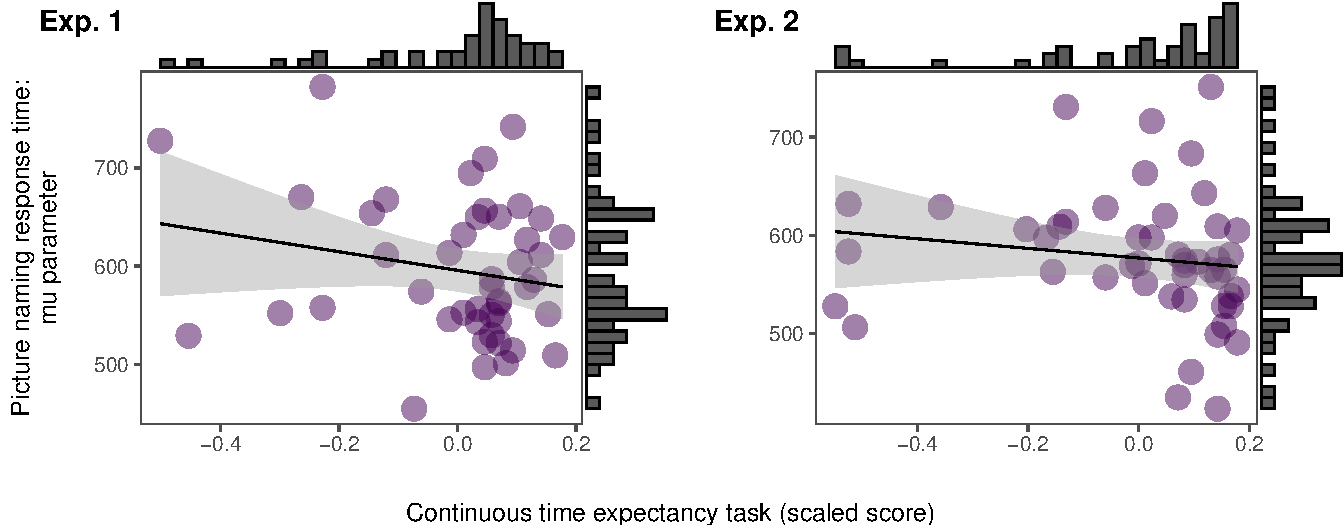
\includegraphics{task_difficulty_ind_dif_files/figure-latex/corr1and2-1.pdf}
\caption{\label{fig:corr1and2}Correlations between the continuous time expectancy task and the \(\mu\) ex-gaussian parameter from participants' picture naming response time distributions in Experiment 1 (left) and the non-speeded condition of Experiment 2 (right).}
\end{figure}

An issue related to statistical power is that of reliability of measures (Parsons, Kruijt, \& Fox, 2019). Recent work has shown that tasks that consistently produce robust experimental effects, such as several conflict tasks thought to measure inhibition (e.g., Flanker, Stroop), have relatively low test-retest reliability (Hedge et al., 2018). That is, participants' scores at one time point are not necessarily highly correlated with their scores at a different time point.

One potential issue in the current study and others that have correlated measures of cognitive skills with picture naming speed is that we currently do not have good estimates of reliability of picture naming measures over time (that we are aware of). Shao and colleagues (2013, 2014, 2012) have reported either split-half reliability (reliability within an experimental session, e.g., the correlation of even and odd experimental trials) or the correlation between two different types of stimuli (actions and objects), and they have typically found high correlations. This is good, but since we do not currently have estimates of test-retest reliability, we do not know, for example, whether the slow speakers in our sample are slow whenever they are tested (i.e., a skill specific to the individual), or if speed of production is a result of other factors such as how tired or alert the individual felt during the testing session. The question of reliability of picture naming measures has theoretical relevance for interpreting correlational studies such as the current study. If we claim that individuals with higher attention or inhibition abilities are faster speakers, we are also making the implicit assumption that these individuals are consistently faster speakers.

Having estimates of reliability is also crucial for questions of sample size and statistical power for correlational studies. For instance, if we correlate two measures that each have relatively low reliability (and likely also high measurement error), this will limit the magnitude of correlations we can find \emph{between} the two measures. If we take the one significant correlation we found in Experiment 1, which was -.31 (assuming this is the true effect size), and we assume each measure (sustained attention and the mu parameter of the picture naming response time distribution) has a reliability of .8, we would still need a sample size of 124 to detect a significant correlation with 80\% power at an alpha level of .05 (Hedge et al., 2018; Parsons et al., 2019). This is much larger than typical sample sizes in this field of research, so it is imperative that future work take issues such as reliability into consideration. We are currently working on a project to establish reliability of picture naming measures.

Finally, there simply might not be strong relationships between measures of cognitive skills and picture naming speed. Of course a non-significant correlation does not mean there is \emph{no} relationship between the measures. Nonetheless, it is possible that any true relationships between these skills are very small, and there may be more effective ways to understand the involvement of cognitive skills or resources in language production. Naming a picture presented on a screen is a fairly simple task, and the cognitive skills or resources needed to complete this task may not be the same ones involved in, for instance, an operation span task, in which participants have to keep words or letters in mind while solving math problems. More ecologically valid experimental settings, such as speaking and driving simultaneously, may be a promising avenue for better understanding the involvement of cognitive skills or resources in speaking (e.g., Becic et al., 2010; Dromey \& Simmons, 2019; Kubose et al., 2006).

\hypertarget{conclusions}{%
\section{Conclusions}\label{conclusions}}

Our aim in this study was to build on previous work showing that measures of working memory, inhibition, and attention correlate with picture naming speed. Specifically, we tested whether we would see significant relationships between picture naming speed and measures from a wider battery of cognitive tasks that tap into different components of these cognitive skills. We found one significant correlation but did not replicate this in a second experiment. We argue that we need better estimates of reliability of picture naming for testing for correlations with other skills, as well as more ecologically valid paradigms for testing the necessity of cognitive skills while speaking.

\clearpage

\hypertarget{references}{%
\section{References}\label{references}}

\hypertarget{refs}{}
\begin{CSLReferences}{1}{0}
\leavevmode\vadjust pre{\hypertarget{ref-baddeley1992working}{}}%
Baddeley, A. (1992). Working memory. \emph{Science}, \emph{255}(5044), 556--559.

\leavevmode\vadjust pre{\hypertarget{ref-baddeley2010working}{}}%
Baddeley, A. (2010). Working memory. \emph{Current Biology}, \emph{20}(4), R136--R140.

\leavevmode\vadjust pre{\hypertarget{ref-balota2011moving}{}}%
Balota, D. A., \& Yap, M. J. (2011). Moving beyond the mean in studies of mental chronometry: The power of response time distributional analyses. \emph{Current Directions in Psychological Science}, \emph{20}(3), 160--166.

\leavevmode\vadjust pre{\hypertarget{ref-becic2010brief}{}}%
Becic, E., Dell, G. S., Bock, K., Garnsey, S. M., Kubose, T., \& Kramer, A. F. (2010). BRIEF REPORTS driving impairs talking. \emph{Psychonomic Bulletin \& Review}, \emph{17}(1), 15--21.

\leavevmode\vadjust pre{\hypertarget{ref-burki2017electrophysiological}{}}%
Bürki, A. (2017). Electrophysiological characterization of facilitation and interference in the picture-word interference paradigm. \emph{Psychophysiology}, \emph{54}(9), 1370--1392.

\leavevmode\vadjust pre{\hypertarget{ref-burki2020did}{}}%
Bürki, A., Elbuy, S., Madec, S., \& Vasishth, S. (2020). What did we learn from forty years of research on semantic interference? A bayesian meta-analysis. \emph{Journal of Memory and Language}, \emph{114}, 104125.

\leavevmode\vadjust pre{\hypertarget{ref-burki2022picture}{}}%
Bürki, A., \& Madec, S. (2022). Picture-word interference in language production studies: Exploring the roles of attention and processing times. \emph{Journal of Experimental Psychology: Learning, Memory, and Cognition}.

\leavevmode\vadjust pre{\hypertarget{ref-conway2005working}{}}%
Conway, A. R., Kane, M. J., Bunting, M. F., Hambrick, D. Z., Wilhelm, O., \& Engle, R. W. (2005). Working memory span tasks: A methodological review and user's guide. \emph{Psychonomic Bulletin \& Review}, \emph{12}(5), 769--786.

\leavevmode\vadjust pre{\hypertarget{ref-corsi1972human}{}}%
Corsi, P. M. (1972). \emph{Human memory and the medial temporal region of the brain.}

\leavevmode\vadjust pre{\hypertarget{ref-de1995strategies}{}}%
De Jong, R., Coles, M. G., \& Logan, G. D. (1995). Strategies and mechanisms in nonselective and selective inhibitory motor control. \emph{Journal of Experimental Psychology: Human Perception and Performance}, \emph{21}(3), 498.

\leavevmode\vadjust pre{\hypertarget{ref-draheim2018item}{}}%
Draheim, C., Harrison, T. L., Embretson, S. E., \& Engle, R. W. (2018). What item response theory can tell us about the complex span tasks. \emph{Psychological Assessment}, \emph{30}(1), 116.

\leavevmode\vadjust pre{\hypertarget{ref-dromey2019bidirectional}{}}%
Dromey, C., \& Simmons, K. (2019). Bidirectional interference between simulated driving and speaking. \emph{Journal of Speech, Language, and Hearing Research}, \emph{62}(7), 2053--2064.

\leavevmode\vadjust pre{\hypertarget{ref-dunabeitia2018multipic}{}}%
Duñabeitia, J. A., Crepaldi, D., Meyer, A. S., New, B., Pliatsikas, C., Smolka, E., \& Brysbaert, M. (2018). MultiPic: A standardized set of 750 drawings with norms for six european languages. \emph{Quarterly Journal of Experimental Psychology}, \emph{71}(4), 808--816.

\leavevmode\vadjust pre{\hypertarget{ref-engle1999working}{}}%
Engle, R. W., Tuholski, S. W., Laughlin, J. E., \& Conway, A. R. (1999). Working memory, short-term memory, and general fluid intelligence: A latent-variable approach. \emph{Journal of Experimental Psychology: General}, \emph{128}(3), 309.

\leavevmode\vadjust pre{\hypertarget{ref-ferreira2002central}{}}%
Ferreira, V. S., \& Pashler, H. (2002). Central bottleneck influences on the processing stages of word production. \emph{Journal of Experimental Psychology: Learning, Memory, and Cognition}, \emph{28}(6), 1187.

\leavevmode\vadjust pre{\hypertarget{ref-forstmann2008function}{}}%
Forstmann, B. U., Jahfari, S., Scholte, H. S., Wolfensteller, U., Wildenberg, W. P. van den, \& Ridderinkhof, K. R. (2008). Function and structure of the right inferior frontal cortex predict individual differences in response inhibition: A model-based approach. \emph{Journal of Neuroscience}, \emph{28}(39), 9790--9796.

\leavevmode\vadjust pre{\hypertarget{ref-foster2015shortened}{}}%
Foster, J. L., Shipstead, Z., Harrison, T. L., Hicks, K. L., Redick, T. S., \& Engle, R. W. (2015). Shortened complex span tasks can reliably measure working memory capacity. \emph{Memory \& Cognition}, \emph{43}(2), 226--236.

\leavevmode\vadjust pre{\hypertarget{ref-fuhrmeister2022distributional}{}}%
Fuhrmeister, P., \& Bürki, A. (2022). Distributional properties of semantic interference in picture naming: Bayesian meta-analyses. \emph{Psychonomic Bulletin \& Review}, \emph{29}(2), 635--647.

\leavevmode\vadjust pre{\hypertarget{ref-fuhrmeister2022behavioral}{}}%
Fuhrmeister, P., Madec, S., Lorenz, A., Elbuy, S., \& Bürki, A. (2022). Behavioral and EEG evidence for inter-individual variability in late encoding stages of word production. \emph{Language, Cognition, and Neuroscience}.

\leavevmode\vadjust pre{\hypertarget{ref-harrison2013working}{}}%
Harrison, T. L., Shipstead, Z., Hicks, K. L., Hambrick, D. Z., Redick, T. S., \& Engle, R. W. (2013). Working memory training may increase working memory capacity but not fluid intelligence. \emph{Psychological Science}, \emph{24}(12), 2409--2419.

\leavevmode\vadjust pre{\hypertarget{ref-hedge2018reliability}{}}%
Hedge, C., Powell, G., \& Sumner, P. (2018). The reliability paradox: Why robust cognitive tasks do not produce reliable individual differences. \emph{Behavior Research Methods}, \emph{50}(3), 1166--1186.

\leavevmode\vadjust pre{\hypertarget{ref-heister2011dlexdb}{}}%
Heister, J., Würzner, K.-M., Bubenzer, J., Pohl, E., Hanneforth, T., Geyken, A., \& Kliegl, R. (2011). dlexDB---eine lexikalische datenbank f{ü}r die psychologische und linguistische forschung. \emph{Psychologische Rundschau}, \emph{62}(1), 10.

\leavevmode\vadjust pre{\hypertarget{ref-hommel1997interactions}{}}%
Hommel, B. (1997). Interactions between stimulus-stimulus congruence and stimulus-response compatibility. \emph{Psychological Research}, \emph{59}(4), 248--260.

\leavevmode\vadjust pre{\hypertarget{ref-jongman2017sustained}{}}%
Jongman, S. R. (2017). Sustained attention ability affects simple picture naming. \emph{Collabra: Psychology}, \emph{3}(1).

\leavevmode\vadjust pre{\hypertarget{ref-jongman2015role}{}}%
Jongman, S. R., Meyer, A. S., \& Roelofs, A. (2015). The role of sustained attention in the production of conjoined noun phrases: An individual differences study. \emph{PloS One}, \emph{10}(9), e0137557.

\leavevmode\vadjust pre{\hypertarget{ref-jongman2015sustained}{}}%
Jongman, S. R., Roelofs, A., \& Meyer, A. S. (2015). Sustained attention in language production: An individual differences investigation. \emph{Quarterly Journal of Experimental Psychology}, \emph{68}(4), 710--730.

\leavevmode\vadjust pre{\hypertarget{ref-klaus2018investigation}{}}%
Klaus, J., \& Schriefers, H. (2018). An investigation of the role of working memory capacity and naming speed in phonological advance planning in language production. \emph{The Mental Lexicon}, \emph{13}(2), 159--185.

\leavevmode\vadjust pre{\hypertarget{ref-kornblum1994way}{}}%
Kornblum, S. (1994). The way irrelevant dimensions are processed depends on what they overlap with: The case of stroop-and simon-like stimuli. \emph{Psychological Research}, \emph{56}(3), 130--135.

\leavevmode\vadjust pre{\hypertarget{ref-kubose2006effects}{}}%
Kubose, T. T., Bock, K., Dell, G. S., Garnsey, S. M., Kramer, A. F., \& Mayhugh, J. (2006). The effects of speech production and speech comprehension on simulated driving performance. \emph{Applied Cognitive Psychology: THe Official Journal of the Society for Applied Research in Memory and Cognition}, \emph{20}(1), 43--63.

\leavevmode\vadjust pre{\hypertarget{ref-laganaro2012time}{}}%
Laganaro, M., Valente, A., \& Perret, C. (2012). Time course of word production in fast and slow speakers: A high density ERP topographic study. \emph{NeuroImage}, \emph{59}(4), 3881--3888.

\leavevmode\vadjust pre{\hypertarget{ref-lehrl1975mehrfachwahl}{}}%
Lehrl, S. (1975). \emph{Mehrfachwahl-wortschatztest MWT-b erlangen}. perimed Verlag.

\leavevmode\vadjust pre{\hypertarget{ref-levelt1999theory}{}}%
Levelt, W. J., Roelofs, A., \& Meyer, A. S. (1999). A theory of lexical access in speech production. \emph{Behavioral and Brain Sciences}, \emph{22}(1), 1--38.

\leavevmode\vadjust pre{\hypertarget{ref-logan1984ability}{}}%
Logan, G. D., \& Cowan, W. B. (1984). On the ability to inhibit thought and action: A theory of an act of control. \emph{Psychological Review}, \emph{91}(3), 295.

\leavevmode\vadjust pre{\hypertarget{ref-lorenz2019age}{}}%
Lorenz, A., Zwitserlood, P., Regel, S., \& Abdel Rahman, R. (2019). Age-related effects in compound production: Evidence from a double-object picture naming task. \emph{Quarterly Journal of Experimental Psychology}, \emph{72}(7), 1667--1681.

\leavevmode\vadjust pre{\hypertarget{ref-massidda2013package}{}}%
Massidda, D., \& Massidda, M. D. (2013). \emph{Package {``retimes''}}.

\leavevmode\vadjust pre{\hypertarget{ref-mathot2012opensesame}{}}%
Mathôt, S., Schreij, D., \& Theeuwes, J. (2012). OpenSesame: An open-source, graphical experiment builder for the social sciences. \emph{Behavior Research Methods}, \emph{44}(2), 314--324.

\leavevmode\vadjust pre{\hypertarget{ref-matzke2018stop}{}}%
Matzke, D., Verbruggen, F., \& Logan, G. (2018). The stop-signal paradigm. \emph{Stevens' Handbook of Experimental Psychology and Cognitive Neuroscience}, \emph{5}, 383--427.

\leavevmode\vadjust pre{\hypertarget{ref-o2009uncovering}{}}%
O'Connell, R. G., Dockree, P. M., Robertson, I. H., Bellgrove, M. A., Foxe, J. J., \& Kelly, S. P. (2009). Uncovering the neural signature of lapsing attention: Electrophysiological signals predict errors up to 20 s before they occur. \emph{Journal of Neuroscience}, \emph{29}(26), 8604--8611.

\leavevmode\vadjust pre{\hypertarget{ref-paap2014bilingual}{}}%
Paap, K. R., \& Sawi, O. (2014). Bilingual advantages in executive functioning: Problems in convergent validity, discriminant validity, and the identification of the theoretical constructs. \emph{Frontiers in Psychology}, \emph{5}, 962.

\leavevmode\vadjust pre{\hypertarget{ref-parsons2019psychological}{}}%
Parsons, S., Kruijt, A.-W., \& Fox, E. (2019). Psychological science needs a standard practice of reporting the reliability of cognitive-behavioral measurements. \emph{Advances in Methods and Practices in Psychological Science}, \emph{2}(4), 378--395.

\leavevmode\vadjust pre{\hypertarget{ref-piai2013working}{}}%
Piai, V., \& Roelofs, A. (2013). Working memory capacity and dual-task interference in picture naming. \emph{Acta Psychologica}, \emph{142}(3), 332--342.

\leavevmode\vadjust pre{\hypertarget{ref-R-base}{}}%
R Core Team. (2021). \emph{R: A language and environment for statistical computing}. Vienna, Austria: R Foundation for Statistical Computing. Retrieved from \url{https://www.R-project.org/}

\leavevmode\vadjust pre{\hypertarget{ref-rey2018inhibition}{}}%
Rey-Mermet, A., \& Gade, M. (2018). Inhibition in aging: What is preserved? What declines? A meta-analysis. \emph{Psychonomic Bulletin \& Review}, \emph{25}(5), 1695--1716.

\leavevmode\vadjust pre{\hypertarget{ref-ridderinkhof2005delta}{}}%
Ridderinkhof, K. R., Scheres, A., Oosterlaan, J., \& Sergeant, J. A. (2005). Delta plots in the study of individual differences: New tools reveal response inhibition deficits in AD/hd that are eliminated by methylphenidate treatment. \emph{Journal of Abnormal Psychology}, \emph{114}(2), 197.

\leavevmode\vadjust pre{\hypertarget{ref-ridderinkhof2004response}{}}%
Ridderinkhof, K. R., Wildenberg, W. P. van den, Wijnen, J., Burle, B., et al. (2004). Response inhibition in conflict tasks is revealed in delta plots. \emph{Cognitive Neuroscience of Attention}, \emph{369}, 377.

\leavevmode\vadjust pre{\hypertarget{ref-rouder2019psychometrics}{}}%
Rouder, J. N., \& Haaf, J. M. (2019). A psychometrics of individual differences in experimental tasks. \emph{Psychonomic Bulletin \& Review}, \emph{26}(2), 452--467.

\leavevmode\vadjust pre{\hypertarget{ref-sarter2001cognitive}{}}%
Sarter, M., Givens, B., \& Bruno, J. P. (2001). The cognitive neuroscience of sustained attention: Where top-down meets bottom-up. \emph{Brain Research Reviews}, \emph{35}(2), 146--160.

\leavevmode\vadjust pre{\hypertarget{ref-scerrati2017comparing}{}}%
Scerrati, E., Lugli, L., Nicoletti, R., \& Umiltà, C. (2017). Comparing stroop-like and simon effects on perceptual features. \emph{Scientific Reports}, \emph{7}(1), 1--11.

\leavevmode\vadjust pre{\hypertarget{ref-shalev2011conjunctive}{}}%
Shalev, L., Ben-Simon, A., Mevorach, C., Cohen, Y., \& Tsal, Y. (2011). Conjunctive continuous performance task (CCPT)---a pure measure of sustained attention. \emph{Neuropsychologia}, \emph{49}(9), 2584--2591.

\leavevmode\vadjust pre{\hypertarget{ref-shao2013selective}{}}%
Shao, Z., Meyer, A. S., \& Roelofs, A. (2013). Selective and nonselective inhibition of competitors in picture naming. \emph{Memory \& Cognition}, \emph{41}(8), 1200--1211.

\leavevmode\vadjust pre{\hypertarget{ref-shao2014electrophysiological}{}}%
Shao, Z., Roelofs, A., Acheson, D. J., \& Meyer, A. S. (2014). Electrophysiological evidence that inhibition supports lexical selection in picture naming. \emph{Brain Research}, \emph{1586}, 130--142.

\leavevmode\vadjust pre{\hypertarget{ref-shao2015selective}{}}%
Shao, Z., Roelofs, A., Martin, R. C., \& Meyer, A. S. (2015). Selective inhibition and naming performance in semantic blocking, picture-word interference, and color--word stroop tasks. \emph{Journal of Experimental Psychology: Learning, Memory, and Cognition}, \emph{41}(6), 1806.

\leavevmode\vadjust pre{\hypertarget{ref-shao2012sources}{}}%
Shao, Z., Roelofs, A., \& Meyer, A. S. (2012). Sources of individual differences in the speed of naming objects and actions: The contribution of executive control. \emph{Quarterly Journal of Experimental Psychology}, \emph{65}(10), 1927--1944.

\leavevmode\vadjust pre{\hypertarget{ref-shipstead2012working}{}}%
Shipstead, Z., Redick, T. S., \& Engle, R. W. (2012). Is working memory training effective? \emph{Psychological Bulletin}, \emph{138}(4), 628.

\leavevmode\vadjust pre{\hypertarget{ref-sikora2016executive}{}}%
Sikora, K., Roelofs, A., Hermans, D., \& Knoors, H. (2016). Executive control in spoken noun-phrase production: Contributions of updating, inhibiting, and shifting. \emph{Quarterly Journal of Experimental Psychology}, \emph{69}(9), 1719--1740.

\leavevmode\vadjust pre{\hypertarget{ref-strayer2001driven}{}}%
Strayer, D. L., \& Johnston, W. A. (2001). Driven to distraction: Dual-task studies of simulated driving and conversing on a cellular telephone. \emph{Psychological Science}, \emph{12}(6), 462--466.

\leavevmode\vadjust pre{\hypertarget{ref-tse2010effects}{}}%
Tse, C.-S., Balota, D. A., Yap, M. J., Duchek, J. M., \& McCabe, D. P. (2010). Effects of healthy aging and early stage dementia of the alzheimer's type on components of response time distributions in three attention tasks. \emph{Neuropsychology}, \emph{24}(3), 300.

\leavevmode\vadjust pre{\hypertarget{ref-unsworth2005automated}{}}%
Unsworth, N., Heitz, R. P., Schrock, J. C., \& Engle, R. W. (2005). An automated version of the operation span task. \emph{Behavior Research Methods}, \emph{37}(3), 498--505.

\leavevmode\vadjust pre{\hypertarget{ref-unsworth2009complex}{}}%
Unsworth, N., Redick, T. S., Heitz, R. P., Broadway, J. M., \& Engle, R. W. (2009). Complex working memory span tasks and higher-order cognition: A latent-variable analysis of the relationship between processing and storage. \emph{Memory}, \emph{17}(6), 635--654.

\leavevmode\vadjust pre{\hypertarget{ref-valente2014erp}{}}%
Valente, A., Bürki, A., \& Laganaro, M. (2014). ERP correlates of word production predictors in picture naming: A trial by trial multiple regression analysis from stimulus onset to response. \emph{Frontiers in Neuroscience}, \emph{8}, 390.

\leavevmode\vadjust pre{\hypertarget{ref-verbruggen2013fictitious}{}}%
Verbruggen, F., Chambers, C. D., \& Logan, G. D. (2013). Fictitious inhibitory differences: How skewness and slowing distort the estimation of stopping latencies. \emph{Psychological Science}, \emph{24}(3), 352--362.

\leavevmode\vadjust pre{\hypertarget{ref-wechsler1987wechsler}{}}%
Wechsler, D. (1987). Wechsler memory scale-revised. \emph{Psychological Corporation}.

\leavevmode\vadjust pre{\hypertarget{ref-wechsler2008wechsler}{}}%
Wechsler, D. (2008). Wechsler adult intelligence scale--fourth edition (WAIS--IV). \emph{San Antonio, TX: NCS Pearson}, \emph{22}(498), 1.

\leavevmode\vadjust pre{\hypertarget{ref-wostmann2013reliability}{}}%
Wöstmann, N. M., Aichert, D. S., Costa, A., Rubia, K., Möller, H.-J., \& Ettinger, U. (2013). Reliability and plasticity of response inhibition and interference control. \emph{Brain and Cognition}, \emph{81}(1), 82--94.

\end{CSLReferences}


\end{document}
